\if c\LaTeXe
\quad
\else

\documentclass{article}

\usepackage{amsmath, amssymb}
\usepackage{comment}
\usepackage{graphicx}
%\usepackage[T1]{fontenc}
%\usepackage{ae, aecompl}
\usepackage[numbers]{natbib}

%%%%%%%%%%%%%%%%%%%%%%%%%%%%%%%%%%%%%%%%%%%%%%%%%%%%%%%%%%%%%%%%%%%%%%%%
%% math

%
% General
%

\DeclareMathOperator{\argmin}{arg\,min}
\DeclareMathOperator{\argmax}{arg\,max}

%
% Sets
%

\newcommand{\card} [1]{{\lvert #1 \rvert}}
\newcommand{\range}[1]{{\left\{ 1, \dots, #1 \right\}}}

%
% Linear algebra
%

\newcommand{\mat}  [1]{{\bf #1}}
\newcommand{\norm} [1]{{\lVert #1 \rVert}}
\newcommand{\vect} [1]{{\mbox{\boldmath $#1$}}}

%
% Probability. The CTAN `proba` package doesn't seem to be that good.
% TODO ensuremath does not seem to be a good idea.
%

\newcommand{\E}    [2]{{\textrm{E} \left[ #1 \mid #2 \right]}}
\newcommand{\LL}   [2]{{\ensuremath{ L \left( #1 \,\middle|\, #2 \right) }}}
\newcommand{\LLL}  [2]{{\ensuremath{ l \left( #1 \,\middle|\, #2 \right) }}}
\newcommand{\N}    [1]{{\ensuremath{ \# \left( \textrm{ #1 } \right) }}}
\newcommand{\PO}   [1]{{\Pr \left( #1 \right)}}
\newcommand{\PP}   [2]{{\PO{ #1 \,\middle|\, #2 }}}

%%%%%%%%%%%%%%%%%%%%%%%%%%%%%%%%%%%%%%%%%%%%%%%%%%%%%%%%%%%%%%%%%%%%%%%%
%% Theoretical computer science

%
% Computational complexity
%

\DeclareMathOperator{\bigO}{O}
\providecommand{\OO}[1]{\bigO\bigl(#1\bigr)}

%%%%%%%%%%%%%%%%%%%%%%%%%%%%%%%%%%%%%%%%%%%%%%%%%%%%%%%%%%%%%%%%%%%%%%%%
%% General text

% \emph toggles italics; \textit sets italics; \em is deprecated
\newcommand{\term} [1]{{\emph{#1\/}}} 

% We don't need to do append a ~ or \ because TeX already handles .,
% correctly. TODO figure out if italics are correct here
\newcommand{\foreign}[1]{{\textit{#1}}}
\newcommand{\ea}      {{\foreign{et~al.}}}
\newcommand{\eg}      {{\foreign{e.g.}}}
\newcommand{\ie}      {{\foreign{i.e.}}}
\newcommand{\TODO} [1]{{\textbf{TODO}: \textit{#1}}}

%%%%%%%%%%%%%%%%%%%%%%%%%%%%%%%%%%%%%%%%%%%%%%%%%%%%%%%%%%%%%%%%%%%%%%%%
%% Remarks. Collected from the pervasive but untraceable `remarks.tex`.

\newif\ifremark
\long\def\remark#1{
\ifremark%
    \begingroup%
    \dimen0=\columnwidth
    \advance\dimen0 by -0.25in%
    \setbox0=\hbox{\parbox[b]{\dimen0}{\protect\em\textcolor{red}{#1}}}
    \dimen1=\ht0\advance\dimen1 by 2pt%
    \dimen2=\dp0\advance\dimen2 by 2pt%
    \vskip 0.25pt%
    \hbox to \columnwidth{%
        \vrule height\dimen1 width 3pt depth\dimen2%
        \hss\copy0\hss%
        \vrule height\dimen1 width 3pt depth\dimen2%
    }%
    \endgroup%
\fi}

\newcommand{\remarkname}[2] {
    \remark{{\bf #1}:#2}
}


\begin{document}

\fi

\section{Low-rank Approximation}

\subsection{Overview}
The goal of the learning algorithm presented in this section is to find a low-rank approximation of the sparse rating matrix 
\begin{equation}
R \approx MU
\end{equation}
where $M$ is a $n_M$-by-$d$ movie property matrix, $U$ is a
$d$-by-$n_U$ user property matrix, and $d$ is the dimension of the
low-rank approximation. Due to the missing entries of $R$, $M$ and $U$
cannot be obtained from singular value decomposition. Instead, the
algorithm learns $M$ and $U$ using linear regression and an EM-like
alternate update algorithm.

The time and space complexity of the algorithm is proportional to
the \textit{sum} of the number of users and movies $(n_U+n_M)$ (not the product!), so it is tractable even for the large data set of the Netflix Prize. However, it strongly overfits to the training data especially when the rating matrix is sparse.

\subsection{Learning Algorithm}

At the beginning of the algorithm, $M$ is randomly initialized and
fixed. Then the $i$-th column of $U$ is learned by regular linear
regression as follows:
\begin{equation}
\vect{u}_i=(\check{M}^T\check{M})^{-1}\check{M}^T \check{\vect r}_i
\label{eq:lrem_core}
\end{equation}
where $\check{\vect r}_i$ is a column vector constructed from the $i$th column of the rating matrix $R$, by excluding the missing elements from it. For example, if the $i$th column of $R$ is $[2 \quad \circ \quad 4 \quad \circ \quad \circ \quad 5 \quad \circ]^T$ where``$\circ$'' means missing element, then $\check{r}_i = [2 \quad 4 \quad 5]^T$. $\check{M}$ is a matrix with the corresponding rows of $M$.

Then in the next step, $U$ is fixed and each row of $M$ is updated in
the exactly same manner. These steps are repeated and $U$ and $M$ are
alternately updated until the training RMSE converges, in a similar
fashion as the EM algorithm.

The important fact is that, by repeating this iteration, the training RMSE monotonically decreases, and eventually converges to the (local) optimum. Linear regression finds the parameter which minimizes the log-likelihood given the following normal distribution with arbitrary fixed variance $\sigma^2$;
\begin{equation}
r_{i,j}\sim N(\vec{m}_i \cdot {\vect u}_j, \sigma^2)
\end{equation}
where $\vec{m}_i$ is the $i$-th row of $M$ and ${\vect u}_j$ is $j$-th column of $U$.

Thus, just as in the EM algorithm, the log-likelihood of the training data monotonically decreases in each iteration. With $\sigma = 1/\sqrt{2}$, the RMSE is exactly the same as the log likelihood. Thus the training RMSE monotonically decreases by iterations.

\subsection{Estimation}
Given the trained matrices $U$ and $M$, the maximum likelihood estimation of the ratings can be easily obtained as follows:
\begin{equation}
\hat{r}_{i,j}=\vec{m}_i \cdot {\vect u}_j.
\end{equation}

Although the actual ratings are given as integer numbers from one to five, the estimations by this algorithm are real numbers. We use the real number outputs without rounding them. However, since ratings are from one to five, the estimations above five are turned into five, and those below one are turned into one. %We call it \textit{rating range correction}\footnote{Is there more appropriate name for this....??}.

\subsection{Result}

We implemented this algorithm in MATLAB as well, and found that it
worked successfully.

Since the initial value of $M$ is randomly chosen, the result is
stochastic. In fact it appears that the result is very sensitive to
the initial value of $M$. Figure~\ref{fig:lrem_typical_plot} shows the
typical result of the training RMSE and the test RMSE as well as the
RMSE when the estimation is simply the average rating of each movie
(i.e. zero-order estimation). The training RMSE monotonically
decreases over iterations as we expected, but the test RMSE does not
necessarily monotonically decrease. There is a large gap between the
training RMSE and test RMSE, indicating that the algorithm strongly
overfits to the training data.

\begin{figure}[ht]
  \begin{center}
    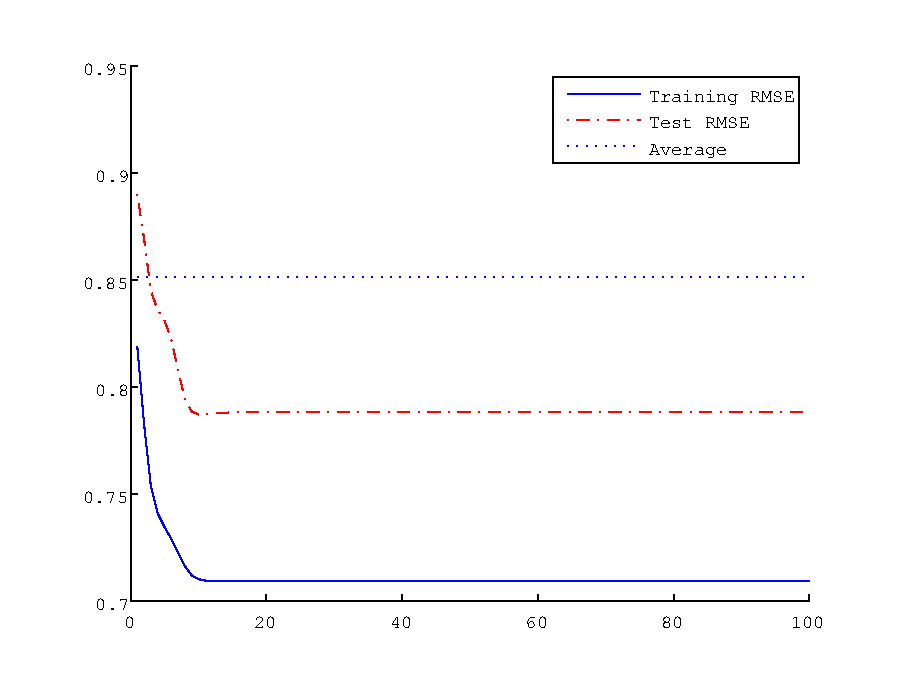
\includegraphics[scale=0.7]{figure/lrem_typical_plot}
  \end{center}
  \caption{Typical result when $d = 2$ and (sparsity ratio)=0.5. The dotted line shows the RMSE when the estimation is simply the average rating of each movie (i.e. zero-order estimation)}
  \label{fig:lrem_typical_plot}
\end{figure}

Table~\ref{table:lrem_result} compares the average RMSE of ten runs
with different dimensions of the low-rank approximation $d$ and
different sparsity ratios. Looking at the table column-wise, we see
that the algorithm works better given training data with fewer missing
ratings, which is an obvious result. An interesting result can be seen
by looking at the table row-wise: a larger dimension results in a
larger RMSE when the rating matrix is sparse, while it results in a
smaller RMSE when the rating matrix is mostly filled. This is because
the algorithm strongly overfits to the training data when the number
of free parameters is large and the number of the available training
data is small.

\begin{table}[ht]
 \caption{RMSE with different dimensions $d$ and different sparsity ratio. The values are the average of ten runs.}
 \label{table:lrem_result}
 \begin{center}
  \begin{tabular}{|c|c||c|c|c|}
    \hline
    \multicolumn{2}{|c|}{}  & \multicolumn{3}{|c|}{Sparsity ratio} \\
    \cline{3-5}
     \multicolumn{2}{|c|}{}    &  0.2 (dense)  &  0.5  & 0.7 (sparse)  \\
    \hline
    \hline
       & 1 &  0.789  &  0.795  &   0.808\\
    \cline{2-5}
     $d$ & 2 &  0.772  &  0.790  & 0.859\\
    \cline{2-5}
     & 3 &  0.772  &  0.808  &    0.933\\
    \hline
  \end{tabular}
 \end{center}
\end{table}

\subsection{Complexity Analysis}
\paragraph{Time complexity} 
The most time-consuming part of the algorithm is the $d$-by-$d$ matrix
inversion $(\check{M}^T\check{M})^{-1}$ in Eq.~\ref{eq:lrem_core}. In
practice, Gaussian elimination, which has a complexity of $\OO{n^3}$,
would be used to find the solution instead of complete matrix
inversion. The inverse of a matrix is computed $(n_U+n_M)$ times in
each iteration. Thus the time complexity of the algorithm is
\begin{equation}
\OO{d^3N(n_U+n_M)}
\end{equation}
where $N$ is the number of iterations.

\paragraph{Space complexity}
Only $U$ and $M$ are stored during computation. Thus the space complexity is
\begin{equation}
\OO{d(n_U+n_M)}.
\end{equation}

\subsection{Estimated performance on the full Netflix Prize data}
\paragraph{Computational cost}
It took about 15 seconds for 100 iterations with $n_U=892$, $n_M=51$,
and $d=3$ on an Intel Celeron 2.0 GHz CPU. For the full data set of
the Netflix Prize, where $n_U=480,189$ and $n_M=17,770$, the
computation for 100 iterations would take about 2 hours with
$d=3$. The required memory space would be about 11 MB. Thus, this is a
tractable algorithm for the full Netflix Prize data.

\paragraph{RMSE}
In the actual Netflix prize data, 99\% of the elements in the rating
matrix are missing. With the small data set where $n_U=892$, $n_M=51$,
the algorithm cannot run with 99\% sparsity ratio since
$(\check{M}^T\check{M})^{-1}$ in Eq.~\ref{eq:lrem_core} becomes
singular for most of the rows due to the lack of data. One thing we
can say for sure from Table~\ref{table:lrem_result} is that the RMSE
would be worse than 0.808 for the full Netflix Prize data set. Trying
the algorithm on the full data is future work.

\subsection{Principle Component Analysis}
Low-rank approximation is equal to the Principle Component Analysis (PCA) when the rating matrix is packed. Thus, by plotting the trained matrix $U$ and $M$ with $d=2$ on 2-D plain, the distribution of user types and movie types can be visualized as Figure \ref{fig:pca}.

\begin{figure}[htbp]
  \begin{center}
    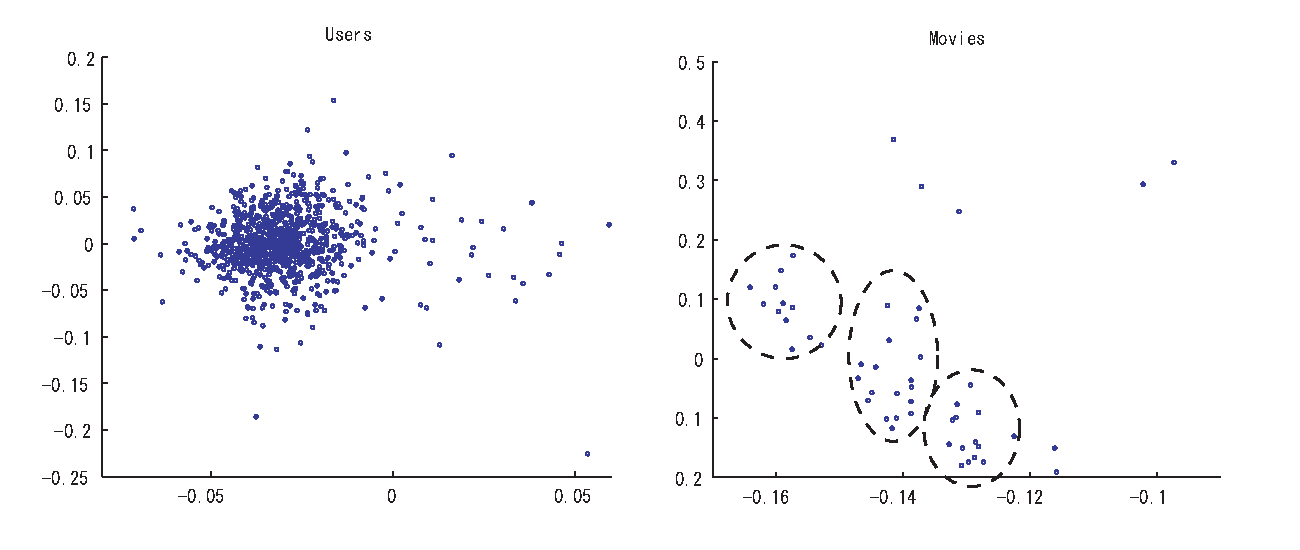
\includegraphics[scale=.75]{figure/pca.eps}
  \end{center}
  \caption{Principle Component Analysis of users and movies, obtained from singular value decomposition of packed rating matrix. Three clusters can be observed in movie domain.}
  \label{fig:pca}
\end{figure}

In the user domain only one cluster is observed, although there are several outliers. On the other hand, three clear clusters can be observed in the movie domain. 

Although low-rank approximation algorithm does not explicitly classify users and movies into discrete types as mixture model, it can captures the latent data structures. 

\subsection{Introducing Prior}
The undesirable behavior of overfitting to the training data may be fixed by introducing the prior belief (in other words, regularization term). As the algorithm overfits to the training data, it tends to give stupid estimations such as $100$ and $-100$, which is reduced to 5 or 1 in the algorithm eventually. If we introduce the prior that forces the predictions for the missing data to stay in the rage $1 \le r \le 5$, result would be improved. This is a future work.


\if c\LaTeXe
\quad
\else
\end{document}
\fi
